% RecallOps Cortex - Project Whitepaper
% Build: tectonic RecallOps-Cortex-Whitepaper.tex  (XeTeX engine)
\documentclass[11pt]{article}

\usepackage{fontspec}
\usepackage[a4paper,margin=2.2cm,headsep=14pt,footskip=26pt]{geometry}
\usepackage{xcolor}
\usepackage{graphicx}
\usepackage{float}
\usepackage{microtype}
\usepackage{parskip}
\usepackage{enumitem}
\usepackage{booktabs}
\usepackage{tabularx}
\usepackage{array}
\usepackage{fancyhdr}
\usepackage{titlesec}
\usepackage{titletoc}
\usepackage{caption}
\usepackage{listings}
\usepackage{tikz}
\usetikzlibrary{positioning,arrows.meta,shapes.geometric}
\usepackage[most]{tcolorbox}
\usepackage[hidelinks]{hyperref}

\graphicspath{{../screens/}}

% ---------------------------------------------------------------- palette ----
\definecolor{ink}{HTML}{0B1020}
\definecolor{panel}{HTML}{121a2e}
\definecolor{cyan}{HTML}{22D3EE}
\definecolor{indigo}{HTML}{6366F1}
\definecolor{amber}{HTML}{F59E0B}
\definecolor{rose}{HTML}{F43F5E}
\definecolor{mint}{HTML}{34D399}
\definecolor{slate}{HTML}{334155}
\definecolor{mutedtext}{HTML}{475569}
\definecolor{rule}{HTML}{E2E8F0}
\definecolor{codebg}{HTML}{0E1526}
\definecolor{codeline}{HTML}{1E293B}

% ----------------------------------------------------------------- fonts -----
\IfFontExistsTF{Calibri}{\setmainfont{Calibri}}{}
\IfFontExistsTF{Segoe UI}{\newfontfamily\headingfont{Segoe UI}}{\let\headingfont\sffamily}
\IfFontExistsTF{Consolas}{\setmonofont[Scale=0.92]{Consolas}}{}

% --------------------------------------------------------------- headings ----
\titleformat{\section}
  {\headingfont\Large\bfseries\color{ink}}
  {\color{cyan}\thesection}{0.7em}{}[\vspace{2pt}{\color{rule}\titlerule[1.2pt]}]
\titleformat{\subsection}
  {\headingfont\large\bfseries\color{indigo}}
  {\thesubsection}{0.6em}{}
\titleformat{\subsubsection}
  {\headingfont\normalsize\bfseries\color{slate}}
  {}{0em}{}
\titlespacing*{\section}{0pt}{20pt}{8pt}
\titlespacing*{\subsection}{0pt}{14pt}{4pt}

% ----------------------------------------------------------------- toc -------
\titlecontents{section}[2.6em]{\addvspace{4pt}\headingfont\bfseries}
  {\contentslabel{2.2em}}{}{\titlerule*[0.7pc]{.}\contentspage}
\titlecontents{subsection}[4.8em]{\small}
  {\contentslabel{2.6em}}{}{\titlerule*[0.7pc]{.}\contentspage}

% --------------------------------------------------------------- header ------
\pagestyle{fancy}
\fancyhf{}
\renewcommand{\headrulewidth}{0pt}
\renewcommand{\footrulewidth}{0pt}
\fancyfoot[L]{\footnotesize\color{mutedtext}\headingfont RecallOps Cortex}
\fancyfoot[C]{\footnotesize\color{mutedtext}\headingfont Operational memory for recall containment}
\fancyfoot[R]{\footnotesize\color{mutedtext}\headingfont\thepage}

% --------------------------------------------------------------- listings ----
\lstdefinestyle{base}{
  backgroundcolor=\color{codebg},
  basicstyle=\ttfamily\footnotesize\color{white!88!cyan},
  keywordstyle=\color{cyan}\bfseries,
  commentstyle=\color{mint!80!white}\itshape,
  stringstyle=\color{amber!90!white},
  numberstyle=\tiny\color{mutedtext},
  showstringspaces=false,
  breaklines=true,
  breakatwhitespace=true,
  columns=fullflexible,
  keepspaces=true,
  frame=single,
  framerule=0pt,
  rulecolor=\color{codeline},
  framexleftmargin=10pt,
  framexrightmargin=8pt,
  framextopmargin=7pt,
  framexbottommargin=7pt,
  xleftmargin=10pt,
  xrightmargin=4pt,
  aboveskip=12pt,
  belowskip=8pt,
}
\lstdefinestyle{py}{style=base,language=Python,morekeywords={async,await,self}}
\lstdefinestyle{js}{style=base,language=Java}
\lstdefinestyle{sql}{style=base,language=SQL,morekeywords={STRING,INT64,BOOL,DISTINCT,COUNTIF}}
\lstdefinestyle{sh}{style=base,language=bash}
\lstset{style=base}

% ----------------------------------------------------------------- boxes -----
\newtcolorbox{factbox}[1][]{
  enhanced,breakable,colback=cyan!6,colframe=cyan!55!indigo,
  boxrule=0.6pt,arc=3pt,left=12pt,right=12pt,top=9pt,bottom=9pt,
  fonttitle=\headingfont\bfseries\color{ink},title={#1}}
\newtcolorbox{honestbox}[1][Reality check]{
  enhanced,breakable,colback=amber!8,colframe=amber!75!black,
  boxrule=0.6pt,arc=3pt,left=12pt,right=12pt,top=9pt,bottom=9pt,
  fonttitle=\headingfont\bfseries\color{ink},title={#1}}
\newtcolorbox{usecase}[1]{
  enhanced,breakable,colback=white,colframe=indigo!70,
  boxrule=0pt,arc=2pt,leftrule=4pt,left=12pt,right=12pt,top=8pt,bottom=10pt,
  borderline west={4pt}{0pt}{indigo},
  fonttitle=\headingfont\bfseries\large\color{ink},title={#1}}
\newtcolorbox{killbox}[1][]{
  enhanced,breakable,colback=ink,colframe=ink,coltext=white,
  arc=4pt,left=14pt,right=14pt,top=11pt,bottom=11pt,
  fonttitle=\headingfont\bfseries\color{cyan},title={#1}}

\newcommand{\route}[1]{{\headingfont\bfseries\color{indigo}#1}}
\newcommand{\code}[1]{{\ttfamily\small #1}}

\setlist[itemize]{leftmargin=1.4em,itemsep=2pt,topsep=3pt}
\setlist[enumerate]{leftmargin=1.6em,itemsep=2pt,topsep=3pt}

\hypersetup{
  pdftitle={RecallOps Cortex - Project Whitepaper},
  pdfauthor={RecallOps Cortex Team},
  colorlinks=true,linkcolor=indigo,urlcolor=cyan!60!indigo,citecolor=indigo}

% ================================================================= TITLE =====
\begin{document}
\begin{titlepage}
\thispagestyle{empty}
\newgeometry{margin=0pt}
\tikz[remember picture,overlay]{\fill[ink] (current page.south west) rectangle (current page.north east);}
\begin{center}
\vspace*{1.6cm}
{\color{cyan}\headingfont\Large CLASS I RECALL \ \textbullet\ \ OPERATIONAL MEMORY ONLINE}\\[1.2cm]

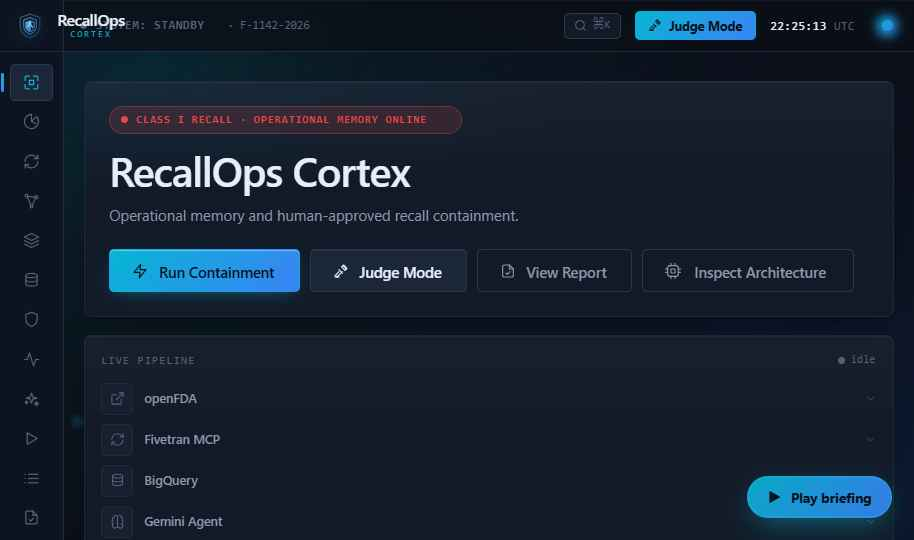
\includegraphics[width=0.82\textwidth]{01-final-premium.png}\\[1.4cm]

{\color{white}\headingfont\fontsize{52}{56}\selectfont\bfseries RecallOps\ \color{cyan}Cortex}\\[10pt]
{\color{white!75!ink}\headingfont\LARGE Operational memory for recall containment}\\[28pt]

{\color{white!70!ink}\large
Turn a real FDA recall into a scoped blast radius, a Gemini drafted action plan,\\
human approvals, and an audit ready compliance report, with a tamper evident trail.}\\[1.4cm]

{\color{cyan}\headingfont\large Google Cloud Rapid Agent Hackathon \ \textbullet\ \ Fivetran Track}\\[6pt]
{\color{white!60!ink}\headingfont MIT Licensed \ \textbullet\ \ June 2026}\\[1.8cm]

{\color{white!55!ink}\small
Live demo \ \textbullet\ \ recall-ops.vercel.app \qquad Repository \ \textbullet\ \ github.com/vaibhav4046/RecallOps}\\[2pt]
{\color{white!40!ink}\footnotesize Project Whitepaper \ \textbullet\ \ goals, use cases, architecture, data model, and operations}
\end{center}
\restoregeometry
\end{titlepage}

\pagecolor{white}

% ================================================================= TOC =======
{\headingfont\hypersetup{linkcolor=ink}
\tableofcontents}
\thispagestyle{fancy}
\clearpage

% ============================================================ 1. SUMMARY =====
\section{Executive summary}

RecallOps Cortex is an agent driven command center for one of the ugliest, highest stakes
problems in food retail: containing a Class I product recall before someone gets hurt and
before a regulator comes asking what you did about it.

A recall lands as a public notice from the FDA. From that single notice, RecallOps Cortex pulls
the real record, scopes it across the retailer's operational data (stores, inventory lots, point
of sale history, in transit shipments, and customer purchase records), and turns it into a
concrete blast radius. It then has Gemini draft a set of containment actions, each one citing the
evidence it is based on. Nothing is executed automatically. A human operator approves every action,
and every approval is written to an append only audit log secured by a sha256 hash chain. The run
ends with an audit ready compliance report and a system state of CONTAINED.

\begin{factbox}[What makes this different from a chatbot]
RecallOps Cortex is not a question and answer box bolted onto a model. It is a real backend
(FastAPI on Cloud Run) wrapping a real workflow: a live recall feed, a queryable warehouse, an
agent that drafts but never executes, a server enforced human approval gate, and a tamper evident
audit trail. The product thesis is blunt: in a regulated workflow, provenance beats autonomy. The
win is not that the machine acts on its own. The win is that every decision is scoped from real
evidence, approved by a human, and provable after the fact.
\end{factbox}

This document explains the project end to end: the problem it attacks, its goals, the people who
would actually use it and the brutal reality of their day, a full tour of the product, the system
architecture, the agent design, the data model, the human approval gate, the audit chain, the
observability layer, the partner ecosystem, the API, security posture, deployment, an honest
account of what is live today versus what activates on deploy, and where it goes next.

% ============================================================ 2. PROBLEM =====
\section{The problem: a recall is chaos on a clock}

When a Class I food recall is issued, it means there is a reasonable probability that the product
will cause serious harm or death. The clock starts immediately. The questions that decide whether
the response is competent or negligent are operational, not philosophical:

\begin{itemize}
\item Which of my locations actually received the affected lots, and how many units are still on the shelf right now?
\item How many units already sold, and to which customers, and did those customers consent to be contacted?
\item Which shipments are in transit at this moment, and which suppliers do I need to put on hold?
\item Which of my stores are highest risk and need to move first?
\item Can I prove, later, exactly what I knew, when I knew it, and what I did about it?
\end{itemize}

In most operations, the answers to those questions live in different systems that do not talk to
each other. Inventory is in a warehouse management system. Sales are in the point of sale platform.
Shipments are in a logistics tool. Customers are in a CRM. The recall notice is a PDF in an inbox.
The actual containment is run out of a spreadsheet, a long email thread, and a panicked group chat,
while a manager reads lot codes off a screen and types them into a search box one at a time.

That manual process is slow, it is error prone, and it leaves a thin and contradictory paper trail.
A missed lot code means contaminated product stays on a shelf. An over broad customer notification
nukes brand trust and buries the call center. A thin audit trail means that when the regulator asks
what happened, the honest answer is a shrug. The Food Safety Modernization Act traceability rule
(commonly referenced as FSMA 204) raises the bar further: operators are expected to produce lot
level traceability records quickly. Spreadsheets do not clear that bar.

\begin{honestbox}[The gap RecallOps Cortex targets]
The bottleneck in a recall is not deciding that a recall is bad. Everyone knows it is bad. The
bottleneck is the frantic, manual, cross system work of figuring out exactly where the blast
radius lands, drafting a coordinated response, getting a human to sign off on each step, and
producing evidence that survives an audit. That is the slice this product owns.
\end{honestbox}

% ============================================================ 3. GOALS =======
\section{Goals and design principles}

\subsection{Product goals}

The objective, taken straight from the build specification, is to operate as a real recall
containment command center that does the following, in order:

\begin{enumerate}
\item Pull an actual food enforcement recall from openFDA, not a scripted demo record.
\item Treat Fivetran synced operational data in BigQuery as the warehouse of record.
\item Use Gemini as the agent brain to reason over the real recall plus the warehouse.
\item Build a blast radius: locations, SKUs, lots, inventory units, sold units, in transit shipments, and the customer notification scope.
\item Draft a complete set of containment actions, each citing its evidence.
\item Require explicit human approval before any external action.
\item Write every decision and approval to an immutable audit log.
\item Generate an audit ready compliance report.
\end{enumerate}

\subsection{Design principles}

\begin{description}[leftmargin=0pt,style=nextline]
\item[Provenance beats autonomy.] The product deliberately refuses to act on its own. Every
externally visible action is drafted, then gated behind a human approval, then logged. For a
regulated workflow this is a feature, not a limitation.
\item[Honest fallback, never a fake green light.] Every integration is badged as live or fallback
based on what actually worked at runtime. openFDA needs no account, so the recall source is live
from the first second. The cloud integrations activate when credentials are present and otherwise
degrade to clearly labelled seeded data so the demo never breaks and never lies.
\item[Real evidence or it does not ship.] Blast radius numbers are computed by aggregating over
rows, not hard coded. In live mode the same aggregation runs as real BigQuery jobs and surfaces
the query job IDs as proof.
\item[Tamper evidence by construction.] The audit log is an append only sha256 hash chain. Altering
any past event breaks every later link, and a verifier re walks the chain to prove integrity.
\item[Command center, not conversation.] The interface is an operations console with fourteen
purpose built routes, not a chat window. The operator sees the recall, the radius, the plan, the
approvals, and the audit at a glance.
\end{description}

% ============================================================ 4. USE CASES ===
\section{Use cases, stated brutally}

Here is the honest version, without the marketing varnish. These are the people who would actually
open this product on the worst morning of their quarter, and what their day looks like with and
without it.

\begin{usecase}{1. The grocery chain buyer who just got the FDA email}
\textbf{Today:} You are a category buyer or a recall coordinator at a regional supermarket chain.
At 7:14am an FDA enforcement notice hits your inbox. You open a spreadsheet, paste in the lot
codes, and start cross referencing them against the warehouse system by hand. You email forty store
managers. You ask IT to block the UPCs at the registers and wait. By the time the stop sale is
actually live, it is mid afternoon and product has been sold all day.

\textbf{With RecallOps Cortex:} You open the command center. The recall is already pulled and
matched. You see exactly which thirty seven locations are affected, that there are 1,842 units to
quarantine and 312 already sold, and a drafted stop sale that names the exact SKUs and lots. You
approve it. The clock that mattered was minutes, not hours.
\end{usecase}

\begin{usecase}{2. The stadium concessions operator mid event}
\textbf{Today:} You run food across dozens of gates at a sold out venue. A recall on a frozen
product drops during the second quarter. You cannot run a spreadsheet during a live event with
sixty thousand people in the building. You radio gate leads and hope.

\textbf{With RecallOps Cortex:} This is the seeded scenario for a reason. The blast radius
separates your six concession gates from the rest of the network, flags the critical tier
locations to move first, and drafts the shelf pull and stop sale per gate. Speed under pressure is
the entire job, and a console beats a radio.
\end{usecase}

\begin{usecase}{3. The pharmacy or drugstore chain with food plus OTC}
\textbf{Today:} You carry food, supplements, and over the counter products, which means recalls hit
you from several directions and the regulators expect lot level precision and a clean record. Your
current process is a patchwork per category.

\textbf{With RecallOps Cortex:} One console, lot level matching, and a tamper evident audit trail
that is built to be handed to a regulator rather than reconstructed after the fact.
\end{usecase}

\begin{usecase}{4. The manufacturer or co-packer issuing the recall}
\textbf{Today:} You are on the supplier side. You initiated the recall and now you owe answers to
your retail customers: which lots, which shipments to divert, which holds to place, and proof that
you notified everyone you were supposed to.

\textbf{With RecallOps Cortex:} The supplier hold and shipment divert actions are first class. The
report bundles the openFDA source, the sync evidence, the queries, the approvals, and the timeline
into something you can actually send.
\end{usecase}

\begin{usecase}{5. The third party logistics and cold chain distributor}
\textbf{Today:} Your exposure is product in motion. Six shipments in transit, three suppliers,
and a receiving dock that needs to know what to quarantine before the truck arrives.

\textbf{With RecallOps Cortex:} The in transit shipment count, the units in motion, and the
supplier holds are computed directly from the warehouse and drafted as divert and hold actions
with the shipments cited as evidence.
\end{usecase}

\begin{usecase}{6. The corporate food safety and compliance team}
\textbf{Today:} You do not run the stores, you answer for them. When an auditor or the FDA asks
what happened, you need a defensible record: who knew what, when, and what they did. Stitching that
together from email after the fact is its own nightmare.

\textbf{With RecallOps Cortex:} The compliance route and the report are the deliverable. The audit
hash chain means the record is not just complete, it is provably unaltered. That is the difference
between evidence and a story.
\end{usecase}

\begin{usecase}{7. The multi location restaurant or QSR franchise}
\textbf{Today:} You need to push a stop sale to independent franchisees and confirm they actually
acted, across a brand you do not directly operate.

\textbf{With RecallOps Cortex:} The action queue assigns owners (store operations, store managers,
procurement, customer care, compliance) so the response is coordinated rather than a broadcast into
the void.
\end{usecase}

\subsection{Who this is NOT for, and what it will not do}

Equally brutal, because a product that claims to be for everyone is for no one:

\begin{itemize}
\item \textbf{Not for a single corner store.} If you have one location, a phone call and a bin bag
beats a command center. The value scales with the number of locations, systems, and customers you
have to coordinate.
\item \textbf{Not a replacement for your WMS, POS, or CRM.} It orchestrates a response across those
systems. It does not run your registers or hold your inventory of record.
\item \textbf{Not autonomous, on purpose.} It will never press the final button for you. If your
goal is a fully automated, no human in the loop pipeline, this is deliberately the wrong tool.
\item \textbf{Only as good as the data you sync.} The blast radius is computed over the operational
warehouse. If the synced data is stale or wrong, the radius is wrong. The product enforces a
freshness check before it will reason, but it cannot invent data you never gave it.
\item \textbf{Scoped to FDA food enforcement today.} The recall source is the openFDA food
enforcement feed. Drug, device, and international recall sources are an extension, not a current
claim.
\end{itemize}

\begin{factbox}[The buyers, named]
The people who sign off on this are a VP or Director of Food Safety, a Director of Store
Operations, a Recall Coordinator, a Compliance Officer, and a Supply Chain Risk Manager. The
trigger to buy is not a feature. It is the memory of the last recall, plus the pressure of FSMA
204 traceability expectations.
\end{factbox}

% ============================================================ 5. TOUR ========
\section{Product tour}

The frontend is a fourteen route command center built with React loaded from a CDN. It hydrates
real backend state on load and badges every integration as live or fallback. Below is the tour,
route by route, with the screens that matter.

\begin{figure}[H]
\centering
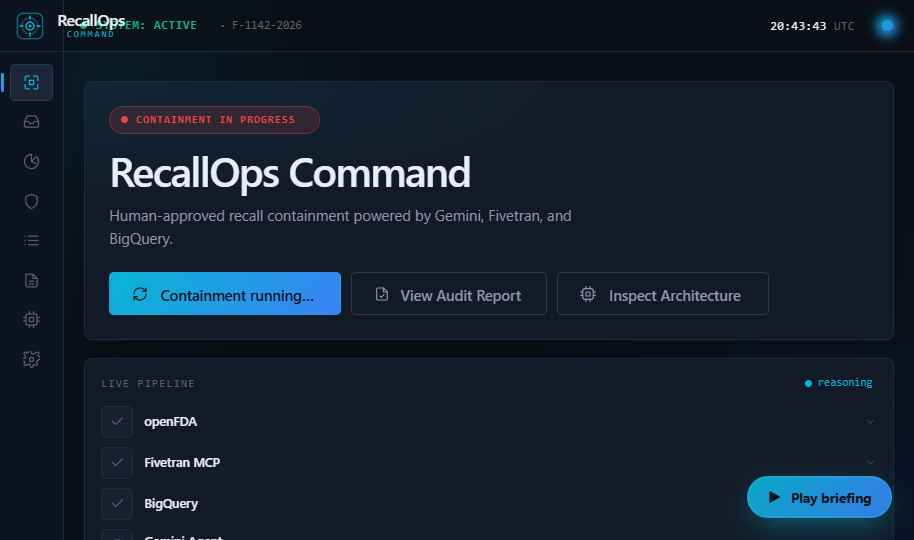
\includegraphics[width=\textwidth]{01-final.png}
\caption{The command center. A single recall, its live blast radius, the drafted plan, and the
system state, all on one console.}
\end{figure}

\subsection{The fourteen routes}

\begin{description}[leftmargin=0pt,style=nextline,itemsep=4pt]
\item[\route{/} command center] The home console. Recall summary, blast radius tiles, agent state, and the path from standby to contained.
\item[\route{/radar} recall radar] openFDA recall intake. Shows the live record id and retrieval time so the source is provably real.
\item[\route{/fivetran} control tower] Connector and sync status across the eight operational sources flowing into BigQuery.
\item[\route{/graph} RecallGraph] The kill shot. A 3D operational memory graph expanding one recall into SKUs, lots, stores, shipments, customers, actions, evidence, and memory.
\item[\route{/context} context pack] The exact bundle handed to the agent: recall, evidence, blast radius, risk rules, and freshness.
\item[\route{/evidence} evidence board] The explainable entity resolution. Deterministic UPC and lot matches scored high, fuzzy product description matches scored lower and routed to human review.
\item[\route{/actions} approval workbench] The human approval queue. Each action opens a pre execution checklist before it can be approved.
\item[\route{/llmops} LLMOps tower] Per run observability: model, prompt version, tool count, latency, token count, and eval score.
\item[\route{/improvement} self improvement] Proposed playbook and memory updates, surfaced only as human approved proposals.
\item[\route{/replay} crisis replay] A replay of the containment timeline for review and training.
\item[\route{/compliance} audit timeline] The append only audit log with its hash chain integrity status.
\item[\route{/report} compliance report] The audit ready bundle: source, sync proof, queries, evidence, approvals, and timeline.
\item[\route{/architecture} architecture] The partner ecosystem and system map, rendered from real backend config.
\item[\route{/settings} settings] Configuration and the secrets stance. No keys in the frontend.
\end{description}

\begin{figure}[H]
\centering
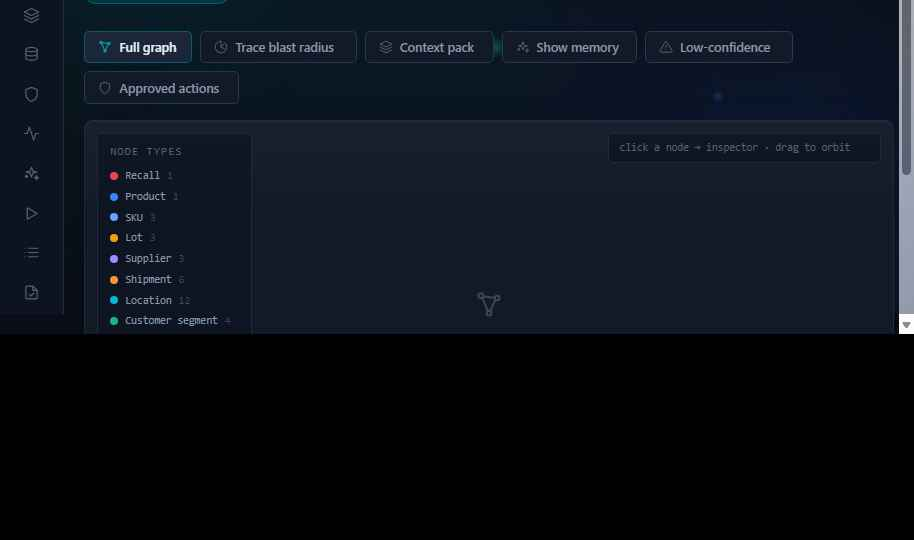
\includegraphics[width=\textwidth]{graph-clean.png}
\caption{RecallGraph. One FDA recall expanded into its full operational neighbourhood: SKUs, lots,
stores, shipments, customers, actions, evidence, and memory.}
\end{figure}

\begin{figure}[H]
\centering
\begin{minipage}{0.49\textwidth}\centering
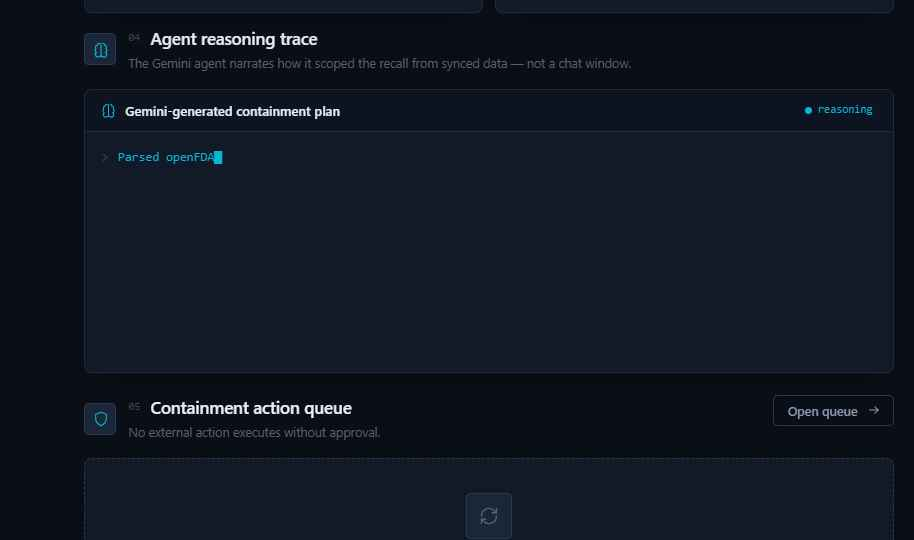
\includegraphics[width=\linewidth]{01-agent.png}
\captionof*{figure}{\small Agent reasoning trace and the drafted action queue.}
\end{minipage}\hfill
\begin{minipage}{0.49\textwidth}\centering
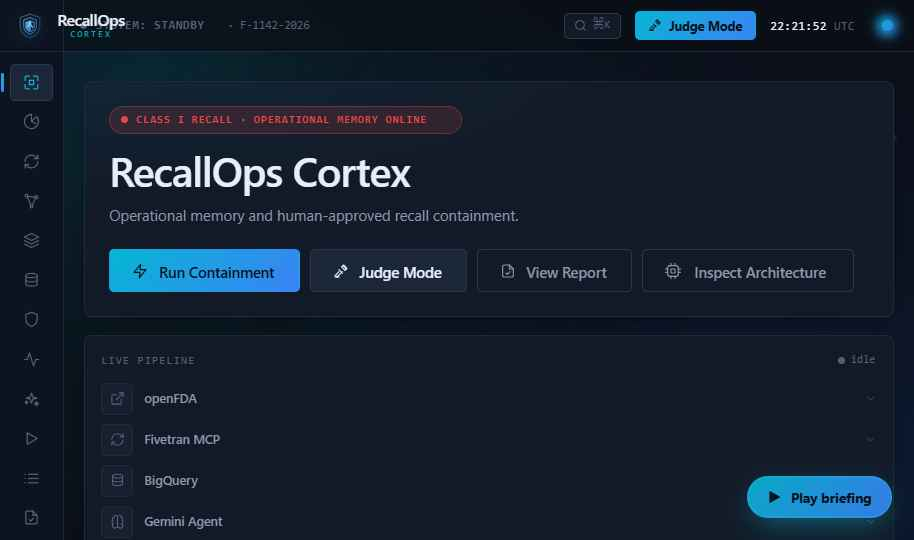
\includegraphics[width=\linewidth]{01-audit-cmd.png}
\captionof*{figure}{\small The audit timeline and command palette.}
\end{minipage}
\caption{Left: the agent narrates how it scoped the recall, then drafts actions for approval.
Right: every step is written to the audit log.}
\end{figure}

% ============================================================ 6. ARCH ========
\section{System architecture}

One Cloud Run service (FastAPI) exposes the structured endpoints the frontend calls. The recall
source is live immediately. The cloud integrations activate when credentials are present and
otherwise fall back to clearly labelled seeded data. Every response carries a trace id.

\begin{figure}[H]
\centering
\resizebox{\textwidth}{!}{%
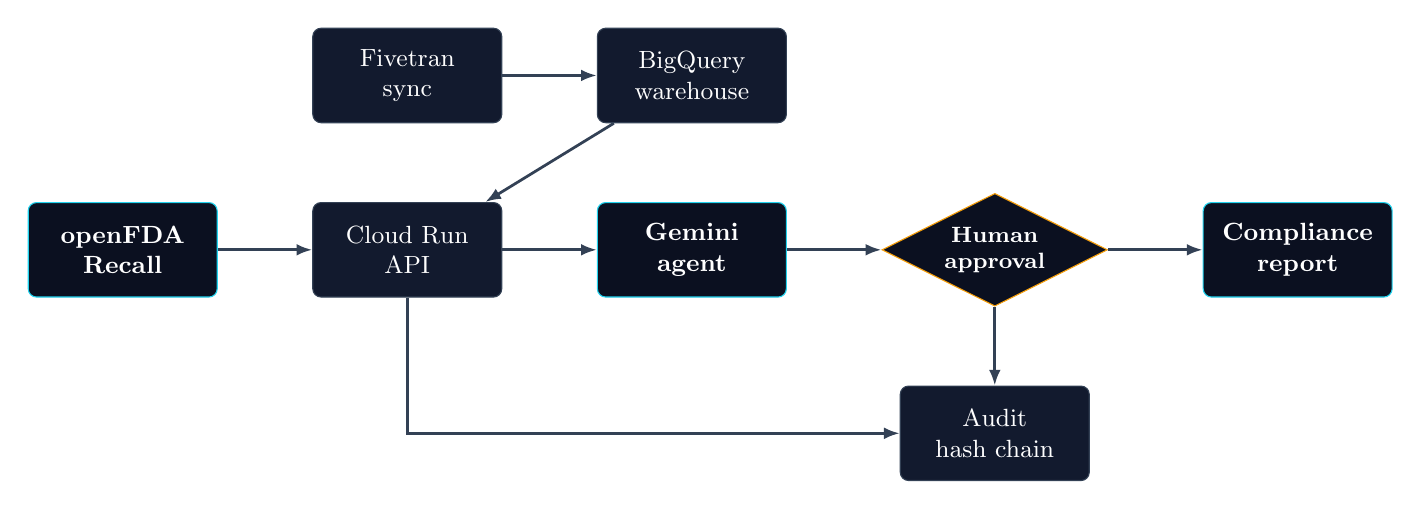
\begin{tikzpicture}[
  node distance=10mm and 12mm,
  box/.style={draw=slate,rounded corners=3pt,fill=panel,text=white,font=\headingfont\small,
    minimum height=12mm,minimum width=24mm,align=center,inner sep=4pt},
  acc/.style={draw=cyan,fill=ink,text=white,rounded corners=3pt,font=\headingfont\small\bfseries,
    minimum height=12mm,minimum width=24mm,align=center},
  gate/.style={draw=amber,fill=ink,text=white,diamond,aspect=2,font=\headingfont\footnotesize\bfseries,
    align=center,inner sep=2pt},
  flow/.style={-{Latex[length=2mm]},draw=slate,line width=1pt}]

\node[acc] (fda) {openFDA\\Recall};
\node[box,right=of fda] (api) {Cloud Run\\API};
\node[box,above=of api] (fiv) {Fivetran\\sync};
\node[box,above right=of api] (bq) {BigQuery\\warehouse};
\node[acc,right=of api] (gem) {Gemini\\agent};
\node[gate,right=of gem] (hum) {Human\\approval};
\node[box,below=of hum] (aud) {Audit\\hash chain};
\node[acc,right=of hum] (rep) {Compliance\\report};

\draw[flow] (fda) -- (api);
\draw[flow] (fiv) -- (bq);
\draw[flow] (bq) -- (api);
\draw[flow] (api) -- (gem);
\draw[flow] (gem) -- (hum);
\draw[flow] (hum) -- (rep);
\draw[flow] (hum) -- (aud);
\draw[flow] (api) |- (aud);
\end{tikzpicture}}
\caption{The agent flow: intake, sync, scope, reason, review, report. The human approval gate sits
between the drafted plan and any external action, and every transition writes an audit event.}
\end{figure}

\subsection{The six phase agent flow}

\begin{enumerate}
\item \textbf{Intake.} Fetch the real openFDA recall and normalise the product description, firm, lot codes, distribution pattern, classification, and reason.
\item \textbf{Sync.} Trigger or validate the Fivetran sync, then confirm warehouse freshness. If the data is older than the configured limit (fifteen minutes), reasoning is blocked.
\item \textbf{Scope.} Query the warehouse for matching SKUs and lots, then aggregate inventory, sales, shipments, locations, and customers into a blast radius and an evidence list.
\item \textbf{Reason.} Gemini receives a context pack (the recall, the evidence, the blast radius, the risk rules, and prior memory) and drafts action cards only, citing evidence ids for every recommendation.
\item \textbf{Review.} The UI shows the action cards. The approval endpoint writes an audit event and changes status. No external integration fires until a human approves.
\item \textbf{Report.} Generate the compliance report with the recall source, sync proof, queries, evidence, approvals, and the full timeline.
\end{enumerate}

\begin{figure}[H]
\centering
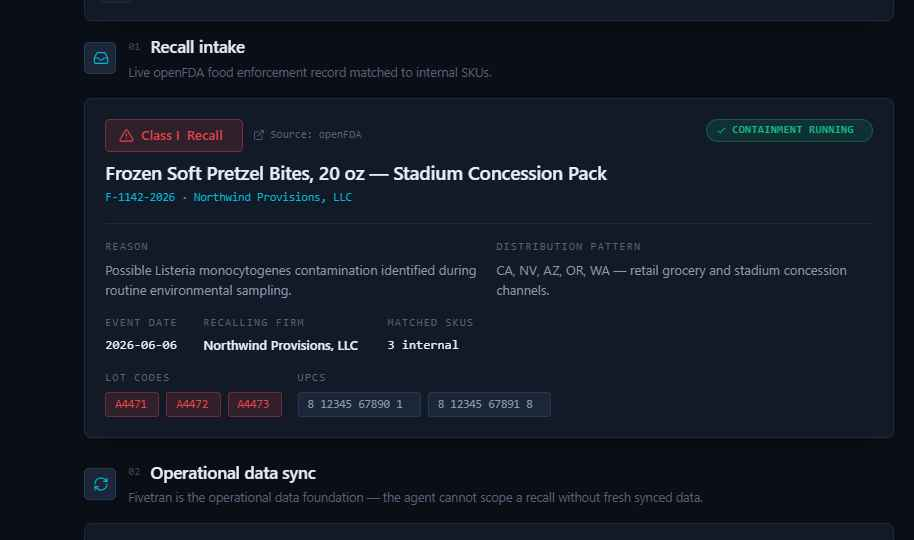
\includegraphics[width=\textwidth]{01-flow.png}
\caption{Data and control flow across the pipeline, as rendered in the product.}
\end{figure}

\subsection{Cloud deployment map}

\begin{center}
\renewcommand{\arraystretch}{1.35}
\begin{tabularx}{\textwidth}{@{}>{\bfseries}l X@{}}
\toprule
Concern & Service \\
\midrule
Frontend & Cloud Run or Vercel (static React) \\
Backend and API & Cloud Run (FastAPI) \\
Agent runtime & Vertex AI Agent Builder or Google ADK \\
Warehouse & BigQuery \\
Data sync & Fivetran plus the Fivetran MCP server \\
Recall source & openFDA Food Enforcement API \\
Secrets & Google Secret Manager \\
Logs & Cloud Logging \\
Reports & Cloud Storage \\
\bottomrule
\end{tabularx}
\end{center}

% ============================================================ 7. AGENT =======
\section{The agent}

The agent is Gemini, and only Gemini. There is no second model and no non Google AI in the running
product. Its job is narrow and explicit: reason over a real recall plus the warehouse, and draft
containment actions. It never executes anything.

\subsection{System prompt and rules}

The agent operates under a fixed system contract. It must reason step by step internally, use tools
before making claims, cite evidence ids for every recommendation, prefer deterministic UPC and lot
matches, lower its confidence for fuzzy product description matches, never execute external actions
without human approval, emit structured JSON, write audit events, and propose self improvements
only as human approved proposals. It must never silently modify production memory or playbooks.

\subsection{The tool layer}

The agent reasons through a fixed tool surface rather than free text:

\begin{center}
\footnotesize\setlength{\tabcolsep}{4pt}
\renewcommand{\arraystretch}{1.25}
\begin{tabularx}{\textwidth}{@{}XXX@{}}
\toprule
Recall and data & Reasoning and graph & Action and audit \\
\midrule
search\_openfda\_recalls & build\_recall\_graph & draft\_containment\_actions \\
get\_recall\_details & get\_graph\_neighbors & submit\_action\_for\_human\_approval \\
trigger\_fivetran\_sync & vector\_search\_similar\_recalls & execute\_approved\_action \\
get\_fivetran\_connector\_status & generate\_context\_pack & write\_audit\_log \\
query\_bigquery & run\_eval\_suite & generate\_compliance\_report \\
\bottomrule
\end{tabularx}
\end{center}

Crucially, \code{execute\_approved\_action} is not callable until a human has moved the action to
the approved state. The model can ask for execution, but the gate lives outside the model.

\subsection{The six canonical actions}

The action \emph{types} are fixed so the command center stays stable and auditable. Gemini (or the
deterministic fallback) writes the human readable draft and the rationale, and the backend computes
the scope from real numbers.

\begin{center}
\renewcommand{\arraystretch}{1.3}
\begin{tabularx}{\textwidth}{@{}>{\bfseries}l l X@{}}
\toprule
Action & Owner & Scope is computed from \\
\midrule
Stop sale & Store Operations & affected locations, SKUs, and inventory units \\
Shelf pull and quarantine & Store Managers & critical tier stores first, then the remainder \\
Supplier hold and divert & Procurement & suppliers and in transit shipments \\
Customer notice & Customer Care & consented customers only, with the rest suppressed \\
Replacement procurement & Procurement & backfill for the critical locations first \\
Compliance report & Compliance & the full recall, evidence bundle, and timeline \\
\bottomrule
\end{tabularx}
\end{center}

\subsection{Live Gemini versus deterministic fallback}

This is the honesty mechanism at the core of the agent. When Gemini credentials are present, the
backend calls the model to write the reasoning trace over the real context pack, and the LLMOps
route shows the real model id, latency, and token counts. When credentials are absent, a
deterministic function produces the same output shape with a clear label so the entire flow stays
demonstrable offline. The output contract is identical in both modes, which is exactly why the
fallback can never masquerade as live: the integration badge reflects what actually ran.

\begin{lstlisting}[style=py,caption={The reasoning call, with a fallback that never breaks the demo (backend/app/gemini.py).}]
def draft_plan(context: dict) -> dict:
    s = get_settings()
    actions = build_actions(context["recall"], context["stats"])
    if not s.gemini_ready:
        return {"reasoning": _fallback_reasoning(...), "actions": actions,
                "model": "deterministic-fallback", "live": False,
                "note": "Gemini not configured - deterministic reasoning (labelled)."}
    resp = client.models.generate_content(
        model=s.gemini_model, contents=prompt,
        config={"response_mime_type": "application/json", "temperature": 0.4})
    return {"reasoning": json.loads(resp.text)["reasoning"], "actions": actions,
            "model": s.gemini_model, "live": True}
\end{lstlisting}

\subsection{The eval suite}

Before a plan is trusted it is checked against a structural eval suite: exact lot match
correctness, UPC match correctness, no customer action without approval, every action has
evidence, a stop sale exists for affected in stock units, a supplier hold exists for in transit
shipments, a customer notice exists for sold units, the compliance report includes a timeline, low
confidence matches require human review, and Fivetran freshness was checked before reasoning.

% ============================================================ 8. DATA ========
\section{Data model}

\subsection{BigQuery warehouse}

The operational warehouse is a small set of BigQuery tables. In fallback mode they are loaded from
the same seed the in process aggregation uses, so live and fallback produce identical numbers. The
difference in live mode is that the aggregation runs as real BigQuery jobs whose job ids are
surfaced as proof.

\begin{lstlisting}[style=sql,caption={Core warehouse table definitions (backend/app/bigquery.py).}]
store_locations(id STRING, name STRING, type STRING, city STRING, manager STRING,
                risk_tier STRING, lot STRING, sku STRING, units INT64)
inventory_lots (location_id STRING, sku STRING, lot STRING, units INT64)
pos_sales      (customer_id STRING, sku STRING, lot STRING, units INT64,
                consented BOOL, channel STRING)
shipments      (id STRING, supplier_id STRING, location_id STRING, sku STRING,
                lot STRING, status STRING, quantity INT64)
recalls_raw    (recall_id STRING, classification STRING, product_description STRING,
                recalling_firm STRING, reason STRING, distribution_pattern STRING,
                event_date STRING, source_url STRING)
\end{lstlisting}

The full warehouse also defines tables for containment actions, approval events, audit events,
agent runs, tool calls, eval results, memory episodes, and improvement proposals, so the entire
agent lifecycle has a durable home.

\subsection{The blast radius query}

The blast radius is a set of aggregations, run as real BigQuery jobs, that reduce the warehouse to
the headline numbers the operator needs.

\begin{lstlisting}[style=sql,caption={Blast radius aggregations (abridged).}]
-- inventory exposure
SELECT COUNT(DISTINCT location_id) locs, SUM(units) units,
       COUNT(DISTINCT sku) skus, COUNT(DISTINCT lot) lots FROM inventory_lots;
-- point of sale exposure and consent split
SELECT SUM(units) units, COUNTIF(consented) consented,
       COUNTIF(NOT consented) suppressed FROM pos_sales;
-- shipments still in motion
SELECT COUNT(*) n, SUM(quantity) units, COUNT(DISTINCT supplier_id) suppliers
       FROM shipments WHERE status = 'in_transit';
-- risk tiered locations
SELECT COUNTIF(risk_tier = 'critical') critical, COUNT(*) total FROM store_locations;
\end{lstlisting}

\begin{factbox}[The seeded scenario, by the numbers]
The reference recall (a Class I Listeria recall on frozen soft pretzel bites) resolves to
37 affected locations, 1,842 inventory units to quarantine, 312 units already sold,
284 consented customers to notify with 41 suppressed for lack of consent, 14 critical tier
locations, 6 shipments in transit across 3 suppliers, and 3 affected SKUs across 3 lots. Every one
of those numbers is aggregated from rows, not typed in by hand.
\end{factbox}

\subsection{Schema contracts}

Three records carry the workflow. A containment action:

\begin{lstlisting}[style=js,caption={containment\_actions record.}]
{ "action_id": "act_1", "recall_id": "F-1142-2026", "type": "STOP_SALE",
  "priority": "critical", "owner": "Store Operations",
  "scope": "37 locations, 3 SKUs, 1842 units", "draft": "Human readable plan",
  "evidence_ids": ["ev_inv", "ev_recall"], "approval_state": "pending",
  "status": "drafted", "created_at": "ISO", "executed_at": null }
\end{lstlisting}

An audit event, which is the link in the hash chain:

\begin{lstlisting}[style=js,caption={audit\_events record.}]
{ "event_id": "au_0001", "recall_id": "F-1142-2026",
  "actor_type": "agent | human | system", "actor_name": "Gemini Agent",
  "event_type": "SYNC_STARTED | QUERY_RUN | ACTION_APPROVED | REPORT_GENERATED",
  "label": "Human approved stop-sale", "evidence_ref": "act_1",
  "timestamp": "ISO", "prev_hash": "...", "hash": "sha256 of (prev_hash + event)" }
\end{lstlisting}

An agent run, which feeds the LLMOps observability:

\begin{lstlisting}[style=js,caption={agent\_runs record.}]
{ "run_id": "run_2042", "recall_id": "F-1142-2026", "model": "gemini-3-pro",
  "prompt_version": "v1.0.0", "tool_count": 12, "latency_ms": 18420,
  "token_count": 41280, "eval_score": 0.94, "status": "passed", "created_at": "ISO" }
\end{lstlisting}

% ============================================================ 9. GATE ========
\section{The human approval gate}

This is the spine of the product, so it is worth being precise about where the gate lives. It is
not a UI convention and it is not a prompt instruction to the model. It is enforced in the backend
orchestrator. The approval function is the only path that can move an action into the executed
state, and it always writes an audit event first. Approving twice is idempotent, so the audit log
never double counts. A recall reaches the contained state only when every drafted action has been
approved.

\begin{lstlisting}[style=py,caption={The approval gate is the only path to execution (backend/app/state.py).}]
def approve_action(self, action_id, actor="Operator", trace_id=""):
    a = self._find_action(action_id)
    if a["approvalState"] == "approved":
        return a                      # idempotent, no duplicate audit event
    a["approvalState"] = "approved"
    a["status"] = "executed"
    a["executedAt"] = _now_iso()
    self.audit.append(recall_id=a["recallId"], actor_type="human", actor_name=actor,
                      event_type="ACTION_APPROVED", label=f'Approved: {a["title"]}',
                      evidence_ref=action_id, phase="approve", trace_id=trace_id)
    return a

def contained(self) -> bool:
    return bool(self.actions) and all(
        a["approvalState"] == "approved" for a in self.actions)
\end{lstlisting}

% ============================================================ 10. AUDIT ======
\section{The tamper evident audit chain}

Every meaningful event, from recall detection to sync to plan drafting to each approval to report
generation, is appended to a hash chain. Each event folds in the previous event's hash, so a
retroactive edit anywhere breaks every link after it. A verifier re walks the chain from a fixed
genesis value and proves whether it is intact. This is the property an auditor actually cares about:
not that you kept a log, but that the log cannot have been quietly rewritten.

\begin{lstlisting}[style=py,caption={The hash chain (backend/app/audit.py).}]
def event_hash(prev_hash: str, event: dict) -> str:
    body = _canonical({k: v for k, v in event.items() if k != "hash"})
    return hashlib.sha256((prev_hash + body).encode("utf-8")).hexdigest()

def verify(self) -> dict:
    prev = self.GENESIS                       # 64 zeroes
    for i, e in enumerate(self._events):
        if e["prev_hash"] != prev or event_hash(prev, e) != e["hash"]:
            return {"intact": False, "broken_at": i, "event_id": e.get("event_id")}
        prev = e["hash"]
    return {"intact": True, "count": len(self._events), "head": prev}
\end{lstlisting}

Events are serialised canonically (sorted keys, fixed separators) before hashing, so the hash is
reproducible regardless of key order. The end to end target is concrete: a real recall, six
approvals, a contained state, and an audit chain that reports intact true.

% ============================================================ 11. OBS ========
\section{Observability and LLMOps}

The agent pipeline is instrumented with OpenTelemetry. Every phase, the BigQuery query, the action
drafting, the eval suite, and the audit write, emits a real span. Spans are captured in process so
the LLMOps route can render a real tool call timeline, and when an OTLP endpoint is configured they
are also exported to any collector. Arize Phoenix is the open source target for LLM tracing and
evals, and Dynatrace is the target for application performance monitoring. The instrumentation is
entirely optional: if the OpenTelemetry packages or the endpoint are absent, every helper degrades
to a no op and the app runs unchanged.

\begin{figure}[H]
\centering
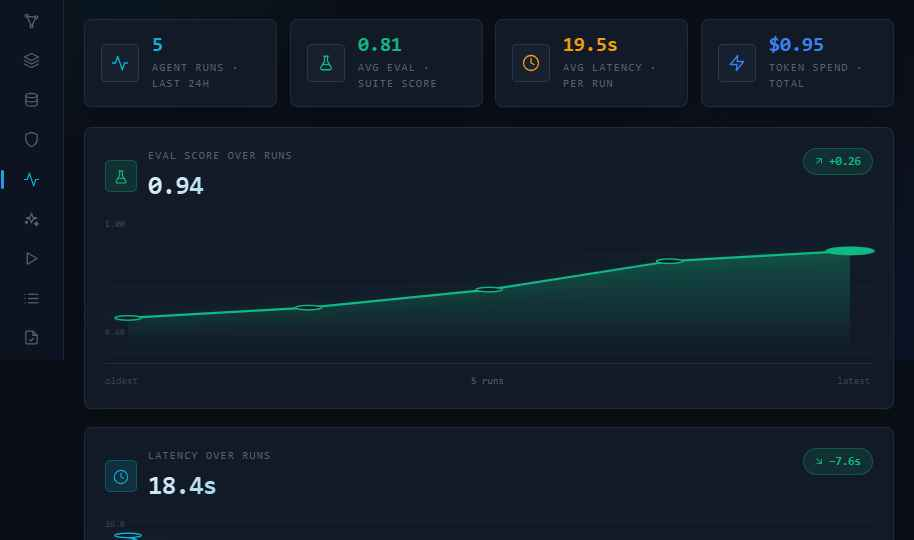
\includegraphics[width=\textwidth]{charts.png}
\caption{The LLMOps tower. Per run model, tool count, latency, token count, and eval score, drawn
from real spans.}
\end{figure}

Each agent run records its model, prompt version, tool count, latency, token count, a structural
eval score, and whether it ran live or in fallback. That record is what makes a run defensible
after the fact rather than a black box.

% ============================================================ 12. PARTNERS ===
\section{Partner ecosystem}

The architecture route renders this map from real backend config. Nothing here is a fake green
light. Each partner is shown as live, pluggable, or in repo based on what is actually wired.

\begin{center}
\renewcommand{\arraystretch}{1.35}
\begin{tabularx}{\textwidth}{@{}>{\bfseries}l X l@{}}
\toprule
Partner & Role & Status \\
\midrule
Google Cloud & Gemini, Agent Builder or ADK, Cloud Run, BigQuery & core \\
Fivetran & Connector sync into BigQuery, plus the Fivetran MCP server as agent tools & live or pluggable \\
Arize Phoenix & LLM tracing and evals over OpenTelemetry & live (open source, local) \\
Dynatrace & Application performance monitoring via OTLP export & otlp ready \\
Elastic & Recall and audit full text search & pluggable adapter \\
MongoDB & Agent memory and vector search over similar recalls & pluggable adapter \\
GitLab & CI and CD with a human gated deploy pipeline & in repo \\
\bottomrule
\end{tabularx}
\end{center}

This breadth is deliberate. The Fivetran track is the chosen lane, and the Fivetran MCP server
wires the same connector operations the agent uses as tools. The observability partners are real
because the pipeline genuinely emits OpenTelemetry. The Elastic and MongoDB adapters are honest
about being pluggable rather than claimed as live.

% ============================================================ 13. API ========
\section{Backend API reference}

One Cloud Run service exposes the structured endpoints below. Every response carries a trace id and
an elapsed time header.

\begin{center}
\renewcommand{\arraystretch}{1.25}
\begin{tabularx}{\textwidth}{@{}l X@{}}
\toprule
Endpoint & Purpose \\
\midrule
\code{GET /api/health} & Mode, integration status, recall id, freshness, and the live Gemini model \\
\code{GET /api/recalls/latest} & Pull the latest real openFDA recall by classification \\
\code{POST /api/recalls/select} & Select a recall and compute its first blast radius \\
\code{POST /api/fivetran/sync} & Trigger a sync (live connectors or labelled fallback) \\
\code{GET /api/fivetran/status} & Connector status, sync timestamp, and freshness \\
\code{POST /api/blast-radius} & Aggregations over the warehouse, with BigQuery job ids in live mode \\
\code{POST /api/agent/run} & Run the agent: context, Gemini draft, eval, audit \\
\code{GET /api/agent/runs} & The run history that feeds LLMOps \\
\code{POST /api/actions/:id/approve} & The approval gate. Writes an audit event and may reach contained \\
\code{POST /api/actions/:id/reject} & Reject an action and log it \\
\code{GET /api/audit/:recallId} & The audit timeline plus a chain integrity verdict \\
\code{POST /api/report/:recallId} & Generate the audit ready compliance report \\
\code{GET /api/ecosystem} & The honest live or pluggable partner map \\
\code{GET /api/state} & One shot hydration snapshot for the frontend \\
\bottomrule
\end{tabularx}
\end{center}

% ============================================================ 14. SECURITY ===
\section{Security and compliance posture}

\begin{itemize}
\item \textbf{No external action without human approval}, enforced server side in the orchestrator rather than in the UI or the prompt.
\item \textbf{Tamper evident audit}, with every step timestamped, attributed to an actor, and chained by sha256. The chain breaks if any event is altered.
\item \textbf{No secrets in the frontend}, repo, logs, or screenshots. Cloud credentials live in Google Secret Manager and are injected at deploy time.
\item \textbf{Honest status by default}, with cached or fallback data clearly labelled and no integration shown as live unless it actually is.
\item \textbf{Freshness gating}, so the agent refuses to reason over warehouse data older than the configured limit.
\end{itemize}

% ============================================================ 15. DEPLOY =====
\section{Deployment}

The app degrades gracefully. Every cloud integration is optional and the service runs in clearly
labelled fallback mode without it. Only the openFDA recall is always live.

\subsection{Run locally, no accounts needed}

\begin{lstlisting}[style=sh,caption={From the repo root.}]
python -m venv .venv
.venv/Scripts/python -m pip install -r backend/requirements.txt
.venv/Scripts/python -m uvicorn app.main:app --app-dir backend --port 8099
python -m http.server 8790          # second terminal, static frontend
\end{lstlisting}

Open the frontend, hit \code{/api/health} to confirm openFDA is live, and run the smoke test, which
should report a pass across the whole flow.

\subsection{Go live}

Going fully live is a sequence of optional steps: add a Gemini key (an AI Studio key is the fastest
path), create a Google Cloud project, stand up the BigQuery dataset and load the warehouse, wire a
Fivetran connector with BigQuery as the destination, deploy the backend to Cloud Run from source,
host the static frontend, and set the api base in the frontend so it points at the deployed service.
At that point health reports live across the board, the LLMOps route shows the real Gemini model and
token counts, the Fivetran route shows real connector status, and the blast radius logs real
BigQuery job ids.

\begin{lstlisting}[style=sh,breakatwhitespace=false,caption={Deploy the backend to Cloud Run from source (no Docker).}]
gcloud run deploy recallops-cortex-api --source backend --region us-central1 \
  --allow-unauthenticated \
  --set-env-vars "GEMINI_MODEL=gemini-3-pro,USE_VERTEX=true,GOOGLE_CLOUD_PROJECT=<id>,BIGQUERY_DATASET=recallops_cortex"
\end{lstlisting}

% ============================================================ 16. HONEST ======
\section{Honest status: live today versus on deploy}

In the spirit of the product's own no fake green lights rule, here is the unvarnished status of the
hosted demo at the time of writing.

\begin{honestbox}[What is real, and what activates on deploy]
\textbf{Real today:} the entire frontend and its fourteen routes, the full FastAPI backend with the
real openFDA client, the real BigQuery adapter and SQL, the sha256 audit chain and its verifier, the
server enforced approval gate, the OpenTelemetry instrumentation, and the deterministic fallback that
keeps the whole flow demonstrable offline. The backend runs end to end locally and passes its smoke
test.

\textbf{Not yet wired on the hosted URL:} the public demo currently serves the frontend in fallback
mode. It is not yet pointed at a deployed Cloud Run backend, so the live openFDA pull, the real
BigQuery job ids, and live Gemini reasoning activate only once the backend is deployed and the api
base is set. The code path for all three exists and is exercised by the backend; what remains is the
deploy and the wiring, not new construction.
\end{honestbox}

This honesty is not a weakness to hide. It is the exact discipline the product preaches, and stating
it plainly is more credible than a glossy claim that a reviewer can disprove by opening the network
tab.

% ============================================================ 17. ROADMAP =====
\section{What is next}

\begin{itemize}
\item Deploy the backend to Cloud Run and point the hosted frontend at it, flipping the live badges on.
\item Multi recall triage, so an operator can run several concurrent recalls from one console.
\item Real notification sandbox integrations, so the customer notice action can execute against a safe test channel rather than only drafting.
\item Richer self improving playbooks under the improvement route, always surfaced as human approved proposals.
\item Extension beyond FDA food enforcement to drug and device recall sources.
\end{itemize}

% ============================================================ 18. VIDEO =======
\section{Appendix A: the three minute demo}

\begin{center}
\renewcommand{\arraystretch}{1.3}
\begin{tabularx}{\textwidth}{@{}l l X@{}}
\toprule
Time & Screen & Beat \\
\midrule
0:00 to 0:20 & command center & A Class I recall just dropped. RecallOps Cortex turns it into a contained, audit ready response. \\
0:20 to 0:40 & recall radar & This is a real openFDA recall, pulled live, with the record id and retrieval time on screen. \\
0:40 to 1:00 & Fivetran control tower & Operational data syncs through Fivetran into BigQuery. The agent will not reason on stale data. \\
1:00 to 1:25 & RecallGraph & One recall expands into SKUs, lots, stores, shipments, and customers. That is the blast radius. \\
1:25 to 1:50 & blast radius and LLMOps & Gemini scopes it: 37 locations, 1,842 units, 312 sold. Every run is instrumented. \\
1:50 to 2:25 & approval workbench & Nothing fires automatically. Each action is gated behind a human approval that writes an immutable audit event. \\
2:25 to 2:45 & compliance timeline & Six approvals, contained. Here is the full timeline. \\
2:45 to 3:00 & compliance report & An audit ready report with a tamper evident hash chain. That is RecallOps Cortex. \\
\bottomrule
\end{tabularx}
\end{center}

% ============================================================ 19. GALLERY =====
\section{Appendix B: screen gallery}

\begin{figure}[H]
\centering
\begin{minipage}{0.49\textwidth}\centering
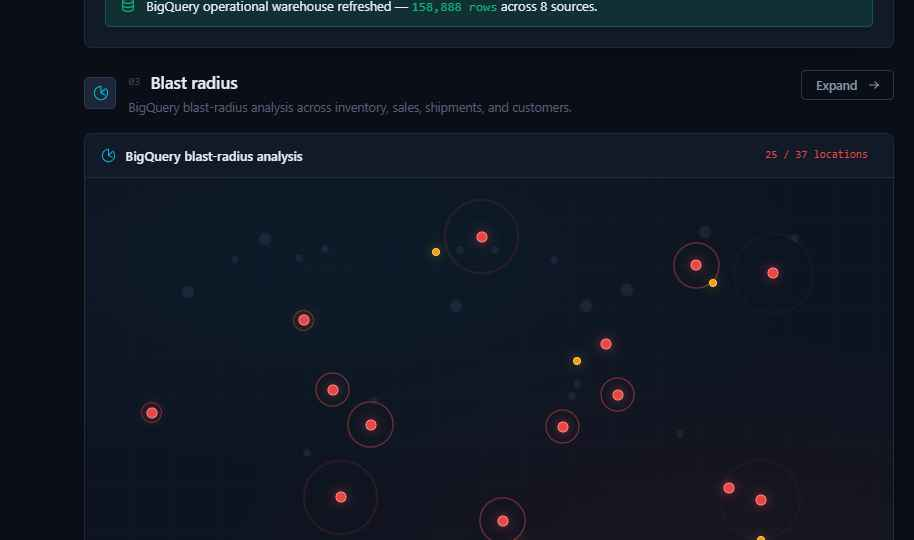
\includegraphics[width=\linewidth]{tiles.png}
\captionof*{figure}{\small Blast radius tiles.}
\end{minipage}\hfill
\begin{minipage}{0.49\textwidth}\centering
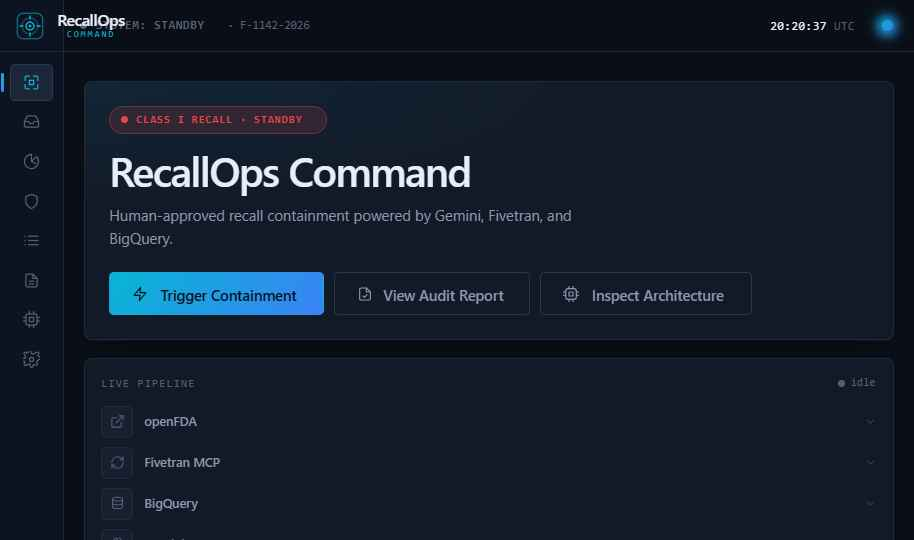
\includegraphics[width=\linewidth]{cmd.png}
\captionof*{figure}{\small The command palette.}
\end{minipage}

\vspace{10pt}
\begin{minipage}{0.49\textwidth}\centering
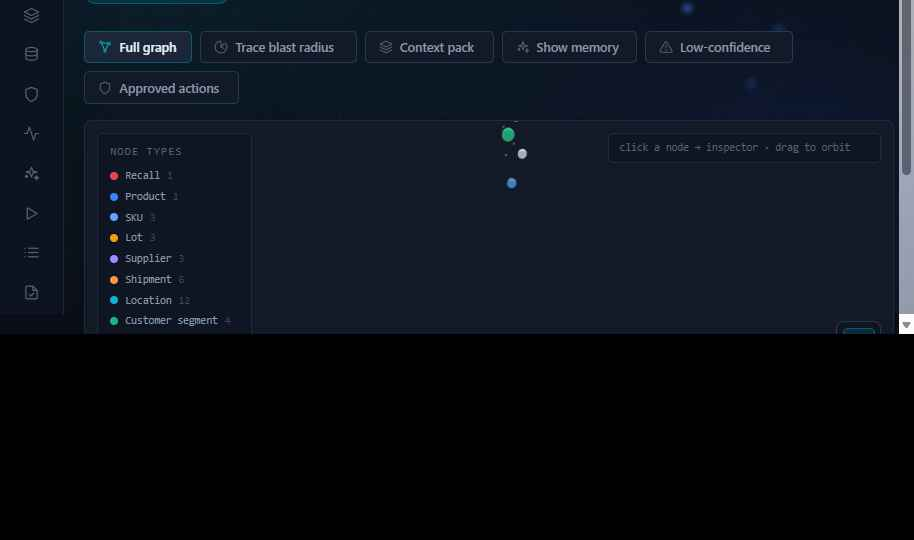
\includegraphics[width=\linewidth]{graph-sleek.png}
\captionof*{figure}{\small RecallGraph, an alternate view.}
\end{minipage}\hfill
\begin{minipage}{0.49\textwidth}\centering
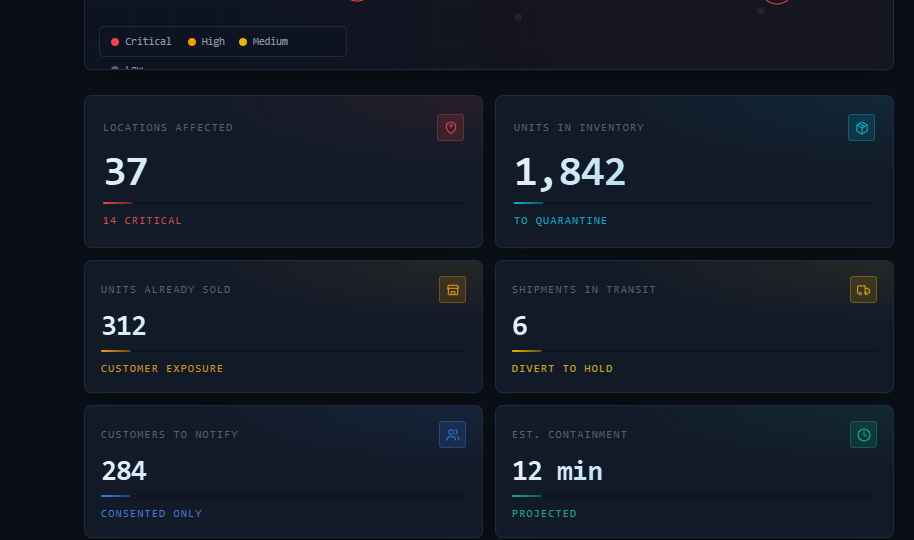
\includegraphics[width=\linewidth]{02-final.png}
\captionof*{figure}{\small The command center in a contained state.}
\end{minipage}

\vspace{10pt}
\begin{minipage}{0.49\textwidth}\centering
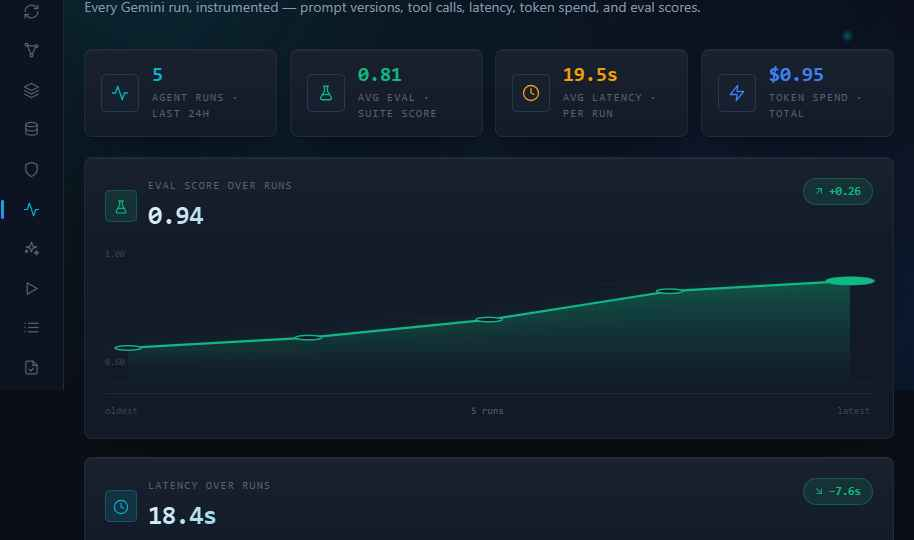
\includegraphics[width=\linewidth]{premium2.png}
\captionof*{figure}{\small Operator console detail.}
\end{minipage}\hfill
\begin{minipage}{0.49\textwidth}\centering
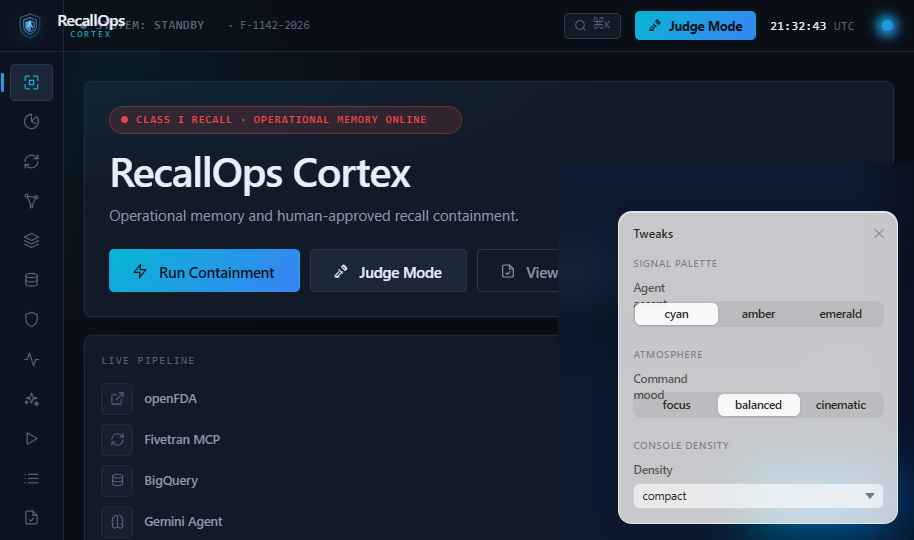
\includegraphics[width=\linewidth]{tweakpanel.png}
\captionof*{figure}{\small Settings and theme controls.}
\end{minipage}
\caption{A selection of the command center surface.}
\end{figure}

\vfill
\begin{center}
{\headingfont\color{mutedtext}\small
RecallOps Cortex \ \textbullet\ \ Operational memory for recall containment \ \textbullet\ \ MIT Licensed\\
github.com/vaibhav4046/RecallOps \ \textbullet\ \ recall-ops.vercel.app}
\end{center}

\end{document}
